\documentclass[tikz,border=8pt]{standalone}
\usepackage{amsmath}
\usetikzlibrary{arrows.meta,calc}
\definecolor{ink}{HTML}{21352F}
\definecolor{teal}{HTML}{087F7B}
\definecolor{blue}{HTML}{4B77A8}
\definecolor{gold}{HTML}{C58B2A}
\definecolor{rose}{HTML}{B65A62}
\begin{document}
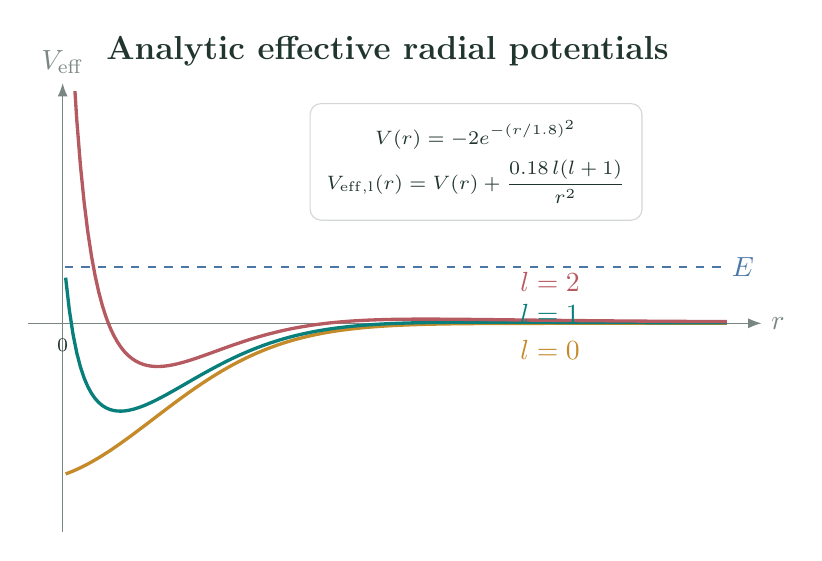
\begin{tikzpicture}[font=\sffamily,text=ink,>=Latex,
                    x=1.25cm,y=1.0cm]
  % Every curve below is generated from
  % V(r)=-2 exp[-(r/1.8)^2] and
  % V_eff,l=V+0.18 l(l+1)/r^2, for r>0.
  \node[font=\bfseries\large] at (3.65,3.45)
    {Analytic effective radial potentials};
  \draw[->,ink!60] (0,0)--(7.45,0) node[right] {$r$};
  \draw[->,ink!60] (.35,-2.65)--(.35,3.05)
    node[above] {$V_{\rm eff}$};
  \node[font=\scriptsize,anchor=north] at (.35,-.08) {$0$};

  \begin{scope}
    \clip (.36,-2.55) rectangle (7.2,2.95);
    \draw[gold,very thick]
      plot[domain=.38:7.1,samples=180,variable=\x]
      (\x,{-2*exp(-(\x/1.8)^2)});
    \draw[teal,very thick]
      plot[domain=.38:7.1,samples=180,variable=\x]
      (\x,{-2*exp(-(\x/1.8)^2)+0.18*2/(\x^2)});
    \draw[rose,very thick]
      plot[domain=.38:7.1,samples=180,variable=\x]
      (\x,{-2*exp(-(\x/1.8)^2)+0.18*6/(\x^2)});
    \draw[blue,dashed,thick] (.37,.72)--(7.1,.72);
  \end{scope}

  \node[gold,anchor=west] at (4.9,-.34) {$l=0$};
  \node[teal,anchor=west] at (4.9,.12) {$l=1$};
  \node[rose,anchor=west] at (4.9,.52) {$l=2$};
  \node[blue,anchor=west] at (7.05,.72) {$E$};

  \node[draw=ink!20,fill=white,rounded corners=4pt,
        align=center,inner sep=6pt,font=\scriptsize] at (4.55,2.05)
    {$\displaystyle V(r)=-2e^{-(r/1.8)^2}$\\[3pt]
     $\displaystyle V_{\rm eff,l}(r)
       =V(r)+\frac{0.18\,l(l+1)}{r^2}$};
\end{tikzpicture}
\end{document}
